\chapter{Asociación con atributo de Enlace}
Es una relación de asociación donde encontramos un atributo que se enlaza con la relación de las clases A - B.
Ese atributo no pertenece ni a la clase A ni a la clase B, si no a la relación.
\begin{figure}[h]
	\centering
	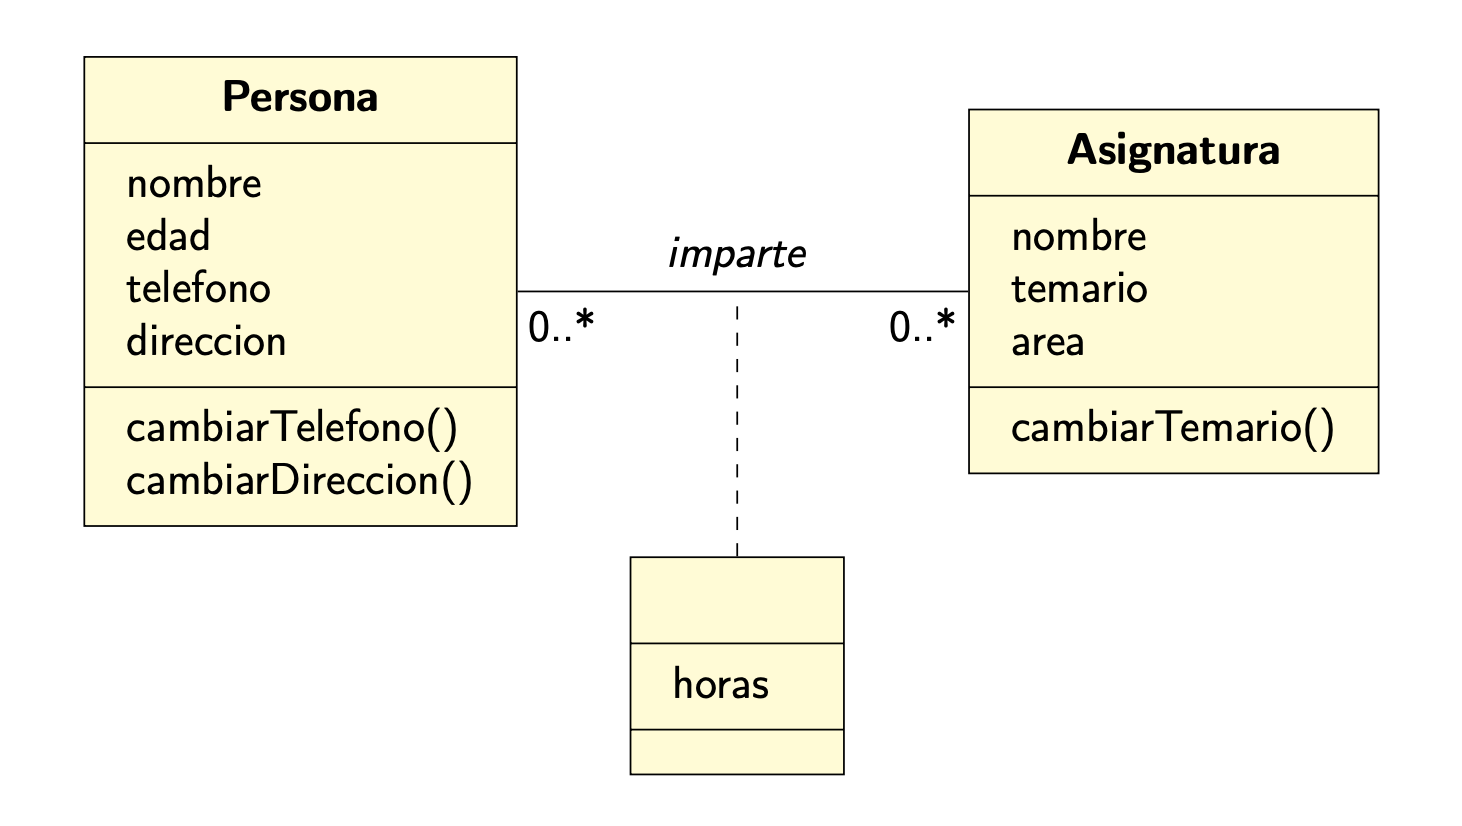
\includegraphics[width=\textwidth]{Imagenes/atribenlace.png}
	\caption{Asociación con atributo de enlace}
\end{figure}

Vemos que una persona imparte asignaturas un número de horas y las asignaturas son impartidas por personas un número de horas.

Dependiendo de la multiplicidad podemos hacer que dicho atributo pertenezca a una de las dos clases (la que tiene mayor multiplicidad).

Si Asignatura tuviera multiplicidad 1, el atributos \textit{horas} iría en la clase Persona → hacemos uso de un conjunto ‘\texttt{set}’.

En este caso, ambos tienen multiplicidad muchos - muchos, por tanto, ese atributo no puede almacenarse en ninguna de las dos clases → tenemos que hacer uso de un diccionario ‘\texttt{map}’.

Como tenemos que las multiplicidad minima es 0, tenemos que hacer si o si una clase de asociación debido a que pueden haber instancias no relacionadas. Por tanto, para las asociaciones con atributo de enlace con multiplicidades \textbf{0..1 - N}, \textbf{0..1 - 1..N} (hacemos clase de asociación o si incluimos en las clases los miembros imprescindibles vamos a tener \texttt{pair<Clase*,atributo>} (en la clase muchos) y un \texttt{map<Clase*, atributo>} en la clase 0..1), en  \textbf{N - M}(podemos hacer una clase de asociación o incluir en ambas clases un \texttt{map<Clase* , atributo>} en ambas)

Si tenemos una relación de este tipo con multiplicidades \textbf{1 - 1} guardamos el atributo de enlace en cualquiera de las dos clases (no en las dos porque sería redundate).

Si tenemos multiplicidades \textbf{1 - N} ó \textbf{1 - 1..N} guardamos el atributo de enlace en la clase con mayor multiplicidad (N ó 1..N) y esta recibe un puntero a la otra clase y la clase con multiplicidad 1 recibe un set de punteros (\texttt{std::set<Clase*>}).
\newpage
\subsection{Implementación de la relación:}

\begin{center}
	\begin{lstlisting}[frame=single]
class Asignatura;
class Persona{
  public:
    typedef std::map<Asignatura*,int> Bs;
    void setA(Asignatura&, int) noexcept;
    const Bs& getB()const noexcept;
  private:
    Bs bs_;
};

class Asignatura{
  public:
    typedef std::map<Persona*,int> As;
    void setB(Persona&, int)noexcept;
    const As& getA()const noexcept;
  private:
    As as_;
};
/*----------Implementacion de los metodos----------*/
void Persona::setA(Asignatura& a, int atributo) noexcept{
  //Sin permitir que se modifique la clave si existe en el diccionario.
  bs_.insert(std::make_pair(&a,atributo));

  //Permite modificar la clave si ya existe en el diccionario.
  //bs_[&a]=atributo;
}

const Persona::Bs& Persona::getB()const noexcept{
  return bs_; 
}

void Asignatura::setB(Persona& p, int atributo)noexcept{
  //No permite que se modifique la clave si existe en el diccionario.
  as_.insert(std::make_pair(&p,atributo));

  //Permite modificar la clave si ya existe en el diccionario.
  //as_[&p]=atributo;
}

const Asignatura::As& Asignatura::getA()const noexcept {
  return as_;
}
\end{lstlisting}
\end{center}